% 冲击波

当波源运动的速度$v_S$超过波的速度$u $时,这时波源将位于波前的前方.如\autoref{ShoWav_fig1}所示.当波源在$A $位置时发出的波,在其后$t $时刻的波阵面为半径等于$ut $的球面,但此时刻波源已前进了$v_St$的距离到达$B $位置,在整个$t $时间内,波源发出的波的各波前的切面形成一个圆锥面,这锥形的顶角满足
\begin{equation}
\sin \alpha=\frac{u t}{v_{\mathrm{s}} t}=\frac{u}{v_{\mathrm{s}}}
\end{equation}
\begin{figure}[ht]
\centering
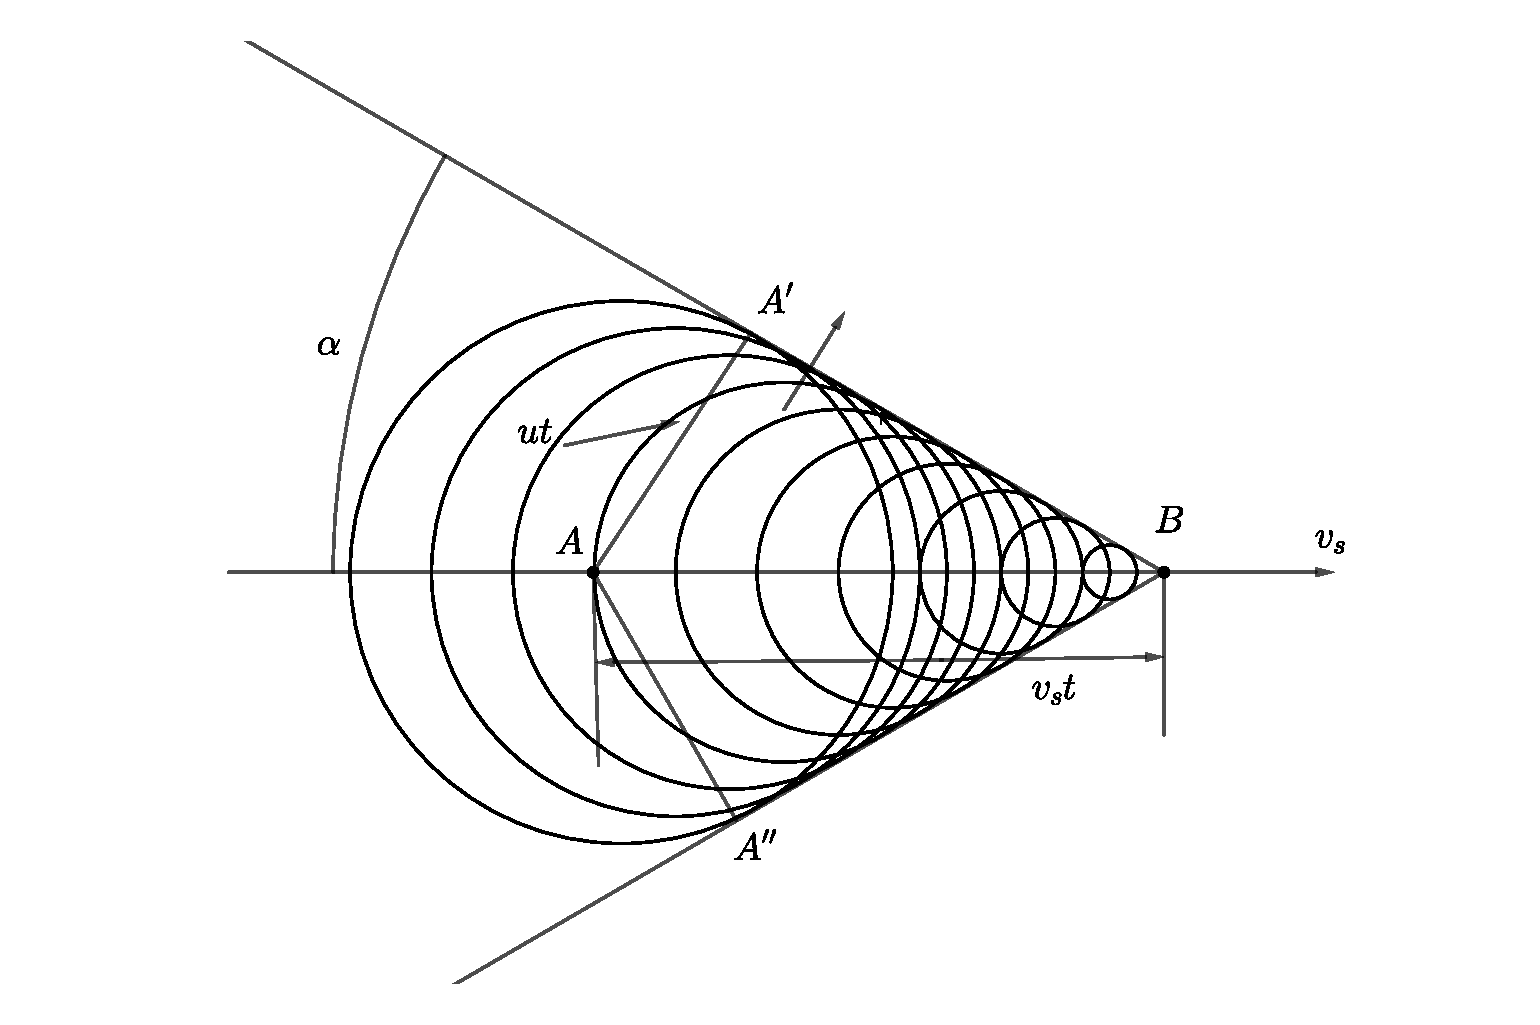
\includegraphics[width=13cm]{./figures/ShoWav_1.pdf}
\caption{冲击波} \label{ShoWav_fig1}
\end{figure}
随着时间的推移,各波前不断扩展,锥面也不断扩展,这种以点波源为顶点的圆锥形的波称为\textbf{冲击波(shock wave)}.$v_S/u$通常称为\textbf{马赫数(Mach number)},$\alpha$称为\textbf{马赫角(Mach angle)}.锥面就是受扰动的介质与未受扰动的介质的分界面,在两侧有着压强、密度和温度的突变.

飞机、炮弹等以超音速飞行时,都会在空气中激起冲击波.过强的冲击波能使掠过地区的物体遭到损坏(如使玻璃窗震碎等),这种现象称为“声暴”.